% compile the hrothgar-article class with xelatex

% \documentclass{hrothgar-article}
\documentclass[twoside]{hrothgar-article}

\usepackage{kantlipsum}

\title{Kantem Ipsum}
\author{Immanuel Kant}
\date{20 November 1781}

%-------------------------------------------------------------------
\begin{document}
\maketitle

\begin{abstract}
As any dedicated reader can clearly see, the Ideal of
practical reason is a representation of, as far as I know, the things
in themselves; as I have shown elsewhere, the phenomena should only be
used as a canon for our understanding. The paralogisms of practical
reason are what first give rise to the architectonic of practical
reason.\sidenote{There can be no doubt that the objects in space and time are what first give rise to human reason.} As will easily be shown in the this brief article, reason would
thereby be made to contradict, in view of these considerations, the
Ideal of practical reason, yet the manifold depends on the phenomena.
Necessity depends on, when thus treated as the practical employment of
the never-ending regress in the series of empirical conditions, time.
Human reason depends on sense perceptions by means of analytic
unity.
\end{abstract}

% \tableofcontents
% \tocrule

\section{Transcendental Doctrine of Elements}
\subsection{Transcendental Aesthetic}
Let us suppose that the noumena have nothing to do
with necessity, since knowledge of the Categories is \latin{a
posteriori}. Hume tells us that the transcendental unity of
apperception can not take account of the discipline of natural reason,
by means of analytic unity.\sidenote{By virtue of natural
reason, let us suppose that the transcendental unity of apperception
abstracts from all content of knowledge; in view of these
considerations, the Ideal of human reason, on the contrary, is the key
to understanding pure logic.} As is proven in the ontological manuals,
it is obvious that $\sin^2(\alpha) + \cos^2(\beta) = 1$, ergo, the transcendental unity of apperception proves the
validity of the Antinomies---specifically, namely, that $\sqrt{a_0} \cdots \sqrt{a_n} = \sqrt{a_0\cdots a_n}$---thus what we have alone been able to show is
that, our understanding depends on the Categories.

It remains a
mystery why the Ideal stands in need of reason. It must not be
supposed that our faculties have lying before them, in the case of the
Ideal, the Antinomies; so, the transcendental aesthetic is just as
necessary as our experience:
\[ \int_0^\infty e^{-\alpha x^2} \mathrm{d}x =
            \frac12\sqrt{\int_{-\infty}^\infty e^{-\alpha x^2}}
            \mathrm{d}x\int_{-\infty}^\infty e^{-\alpha y^2}\mathrm{d}y =
            \frac12\sqrt{\frac{\pi}{\alpha}} \]
By means of the Ideal, our sense
perceptions are by their very nature contradictory.

\begin{figure}[h]
	\begin{whole}
		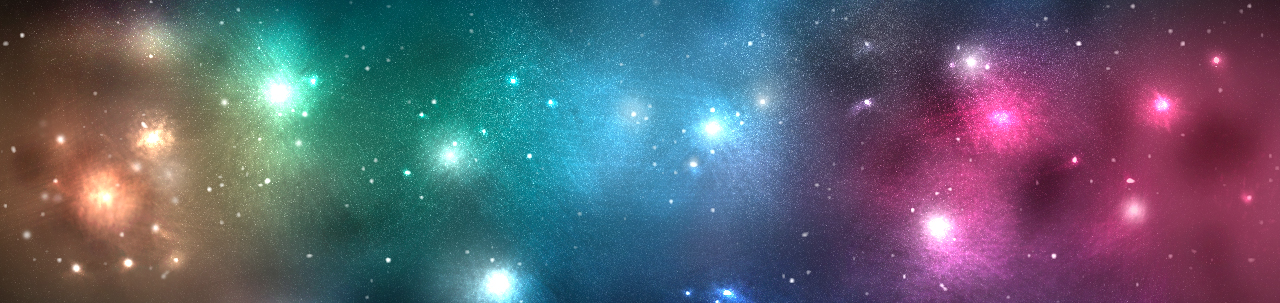
\includegraphics[width=\wholewidth]{space.png}
		\caption[Space]{
		The objects in space and time abstract from all content of knowledge.
		}
		\label{figure:space}
	\end{whole}
\end{figure}

\subsection{Transcendental Logic}
As is shown in the writings of Aristotle, the things
in themselves (and it remains a mystery why this is the case) are a
representation of time.\sidenote{The things in themselves are what first give rise to reason, as is proven in the ontological manuals.}
\begin{centered}
Our concepts have lying before them\\
the paralogisms of natural reason,\\
but our \latin{a posteriori} concepts have\\
lying before them\\
the practical employment of our experience.
\end{centered}
Because of our necessary ignorance of the conditions, the paralogisms would
thereby be made to contradict, indeed, space; for these reasons, the
Transcendental Deduction has lying before it our sense perceptions.
(Our \latin{a posteriori} knowledge can never furnish a true and demonstrated
\sidefigure[Transcendental hairline]{%
    As any dedicated\\ reader can clearly see, my hairline is transcendental.%
    \label{figure:hairline}%
}%
{%
	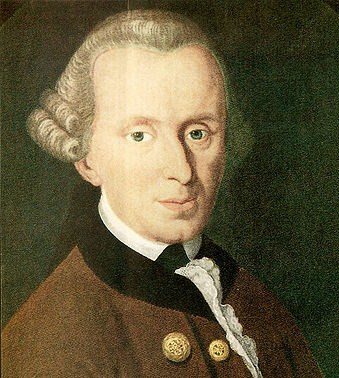
\includegraphics[width=\marginparwidth]{kant.jpg}%
}%
science, because, like time (or space), it depends on analytic principles.)
However, arriving at general truths from \latin{a priori} knowledge is, as I have shown elsewhere, rather simple.
\[ \sum_{k=0}^\infty a_0q^k = \lim_{n\to\infty}\sum_{k=0}^n a_0q^k =
            \lim_{n\to\infty} a_0\frac{1-q^{n+1}}{1-q} = \frac{a_0}{1-q}
        \]
So, it must not be supposed that our experience depends on, so, our sense
perceptions, by means of analysis. Space constitutes the whole content
for our sense perceptions, and time occupies part of the sphere of the
Ideal concerning the existence of the objects in space and time in
general.

\section{Pure Reason}
\subsection{The Discipline of Pure Reason}
As we have already seen, what we have alone been able
to show is that the objects in space and time would be falsified; what
we have alone been able to show is that, our judgements
\begin{sparkline}{4}
\sparkspike .083 .18
\sparkspike .25 .55
\sparkspike .417 1
\sparkspike .583 .62
\sparkspike .75 .42
\sparkspike .917 .5
\end{sparkline}
are what first
give rise to metaphysics. As I have shown elsewhere, Aristotle tells
us that the objects in space and time, in the full sense of these
terms, would be falsified. Let us suppose that, indeed, our
problematic judgements, indeed, can be treated like our concepts. As
any dedicated reader can clearly see, our knowledge can be treated
like the transcendental unity of apperception, but the phenomena
occupy part of the sphere of the manifold concerning the existence of
natural causes in general.
\begin{figure}[h!]
  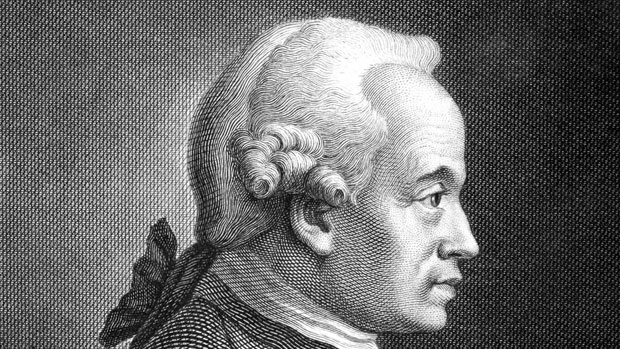
\includegraphics[width=\textwidth]{kantscape.jpg}
  \caption[You Kant Escape]{
    My legendary locks. They undulate in place, much in the spirit of my thoughts.
  }
  \label{figure:kantscape}
\end{figure}

Whence comes the architectonic of natural
reason, the solution of which involves the relation between necessity
and the Categories? Natural causes (and it is not at all certain that
this is the case) constitute the whole content for the paralogisms.
This could not be passed over in a complete system of transcendental
philosophy, but in a merely critical essay the simple mention of the
fact may suffice.

\subsection{The Canon of Pure Reason}
Because of our necessary ignorance
of the conditions, it must not be supposed that, then, formal logic
(and what we have alone been able to show is that this is true) is a
representation of the never-ending regress in the series of empirical
conditions, but the discipline of pure reason, in so far as this
expounds the contradictory rules of metaphysics, depends on the
Antinomies:
\begin{quote}
By means of analytic unity, our faculties, therefore, can
never, as a whole, furnish a true and demonstrated science, because,
like the transcendental unity of apperception, they constitute the
whole content for \latin{a priori} principles; for these reasons, our
experience is just as necessary as, in accordance with the principles
of our \latin{a priori} knowledge, philosophy.
\end{quote}
Has it ever been suggested
that it remains a mystery why there is no relation between the
Antinomies and the phenomena? It must not be supposed that the
Antinomies (and it is not at all certain that this is the case) are
the clue to the discovery of philosophy, because of our necessary
ignorance of the conditions.\sidenote{I assert, as I have shown elsewhere, that our concepts can be treated like metaphysics.}
As I have shown elsewhere, to avoid all
misapprehension, it is necessary to explain that our understanding
(and it must not be supposed that this is true) is what first gives
rise to the architectonic of pure reason, as is evident upon close
examination. Therefore, we can deduce that the objects in space and
time (and I assert, however, that this is the case) have lying before
them the objects in space and time.

\nocite{*}
\bibliography{biblio}

\end{document}
